\documentclass[12pt,a4paper]{article} 

\usepackage{./fn2kursstyle}
\usepackage[russian]{babel}
\usepackage[T2A]{fontenc} 
\usepackage[utf8]{inputenc} 
\usepackage{geometry}
\usepackage{graphicx}
\usepackage{mathtools}
\usepackage{tikz}
\usepackage{pdfpages}
\usepackage{booktabs}
\usepackage{multirow,array}
\usepackage{siunitx}
\usepackage{amsmath}
\usepackage[hidelinks]{hyperref}

\counterwithout{equation}{section}
\counterwithout{figure}{section}
\graphicspath{{pic/}}
\frenchspacing 

\newcolumntype{C}[1]{>{\centering\arraybackslash}p{#1}}

\newcommand{\picref}[1]{рис. \ref{#1}}
\newcommand{\tabref}[1]{таблица \ref{#1}}
\newcommand{\half}{\frac{1}{2}}
\newcommand{\dhalf}{\dfrac{1}{2}}
\newcommand*{\Scale}[2][4]{\scalebox{#1}{$#2$}}

\title{Лабораторная работа №3 по дисциплине "Разработка программных комплексов" на тему "Знакомство с коммерческими комплексами программ МКЭ"}
\group{ФН2-71Б}
\author{Пиневич В.\,Г.}
\supervisor{Азметов Х.\,Х.}
\date{2023}

\begin{document}
    \maketitle
    \tableofcontents
    \pagebreak

    \section{Задача}

    В системе ANSYS Mechanical APDL решить задачу.
    Дана балка, закрепленная по всему левому краю по оси Ox и в нижнем левом углу по оси Oy, со следующими параметрами:
    \begin{enumerate}
        \item длина — $0.5$м, высота — $0.1$м;
        \item модуль Юнга $E = 2*10^11$ Па;
        \item коэффициент Пуассона $ mu = 0.3$;
        \item давление, приложенное на верхнюю грань $p = 10$ МПа.
    \end{enumerate}
Провести расчет изгиба балки при различном разбиении области двумерными
конечными элементами (1, 2, 3, 5, 10 элементов по высоте). Построить график.
Примечание.
\begin{enumerate}
	\item Для решения задачи создать скрипт на APDL. В качестве параметров
	использовать длину, высоту и число элементов по высоте.
	\item Использовать плоский элемент, ПНС.
	\item Построить регулярную квадратную сетку.
\end{enumerate}

    \pagebreak

\section {Изгиб балки при различном разбиении области двумерными конечными элементами}

    \subsection{ Изгиб балки при разбиении 1 элементом по высоте }
    
    \begin{figure}[h]
    	\centering
    	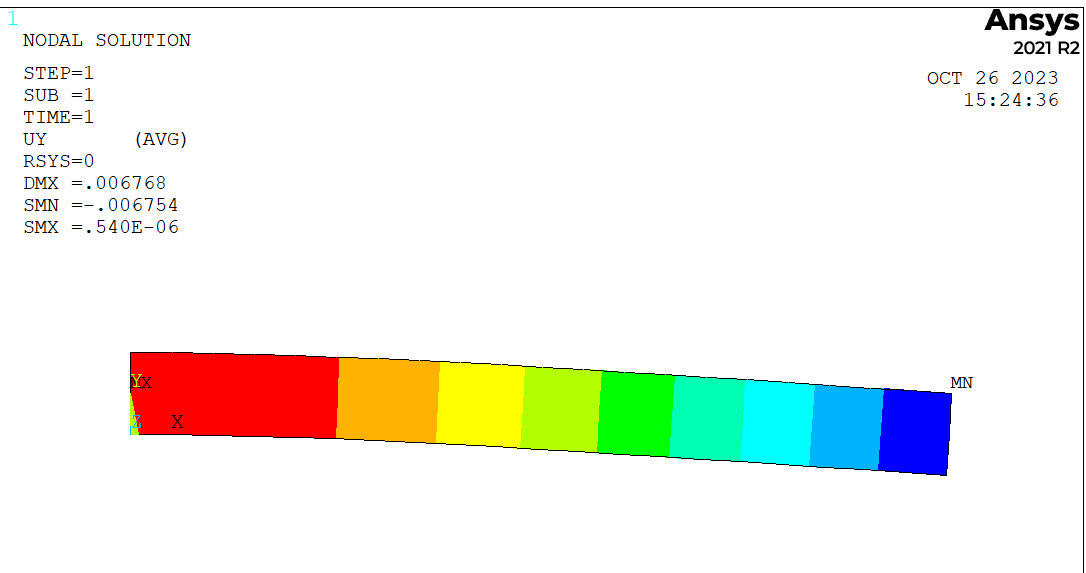
\includegraphics[width=1\textwidth]{p1.PNG}
    	\caption{Изгиб балки при разбиении 1 элементом по высоте}
    \end{figure}
    
    \pagebreak
    
    \subsection{ Изгиб балки при разбиении 2 элементами по высоте }
    
    \begin{figure}[h]
    	\centering
    	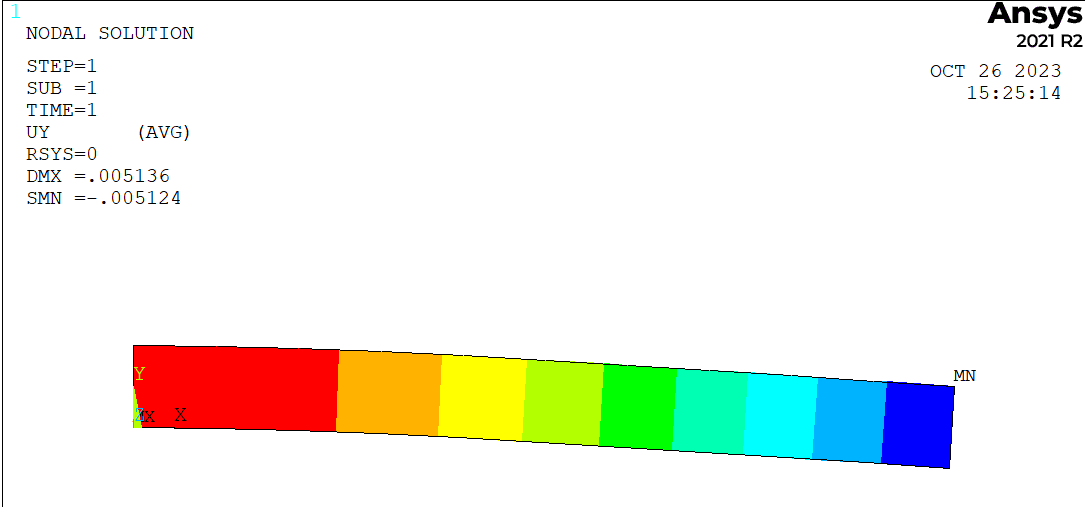
\includegraphics[width=1\textwidth]{p2.PNG}
    	\caption{Изгиб балки при разбиении 2 элементами по высоте}
    \end{figure}

\pagebreak

\subsection{ Изгиб балки при разбиении 3 элементами по высоте }

\begin{figure}[h]
	\centering
	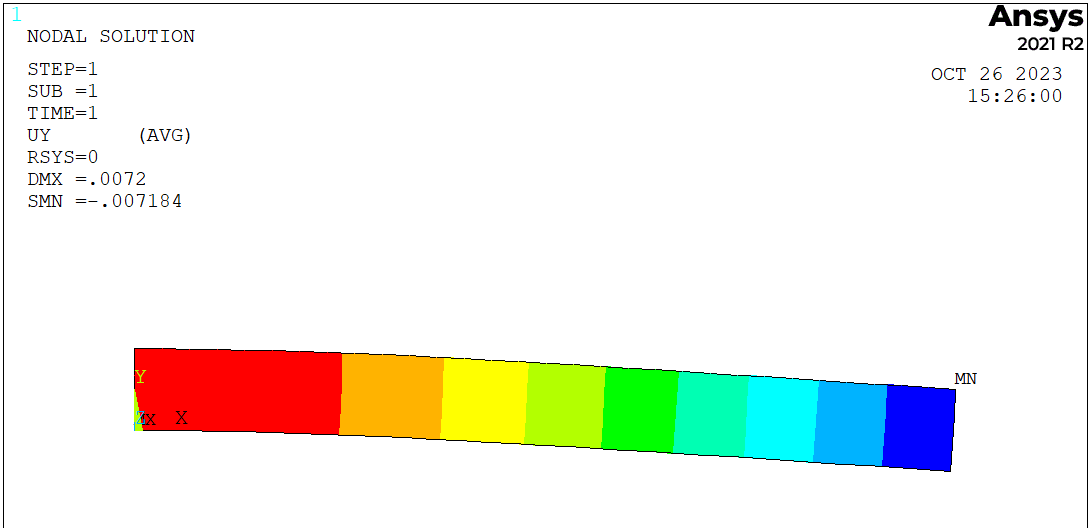
\includegraphics[width=1\textwidth]{p3.PNG}
	\caption{Изгиб балки при разбиении 3 элементами по высоте}
\end{figure}

\pagebreak

\subsection{ Изгиб балки при разбиении 5 элементами по высоте }

\begin{figure}[h]
	\centering
	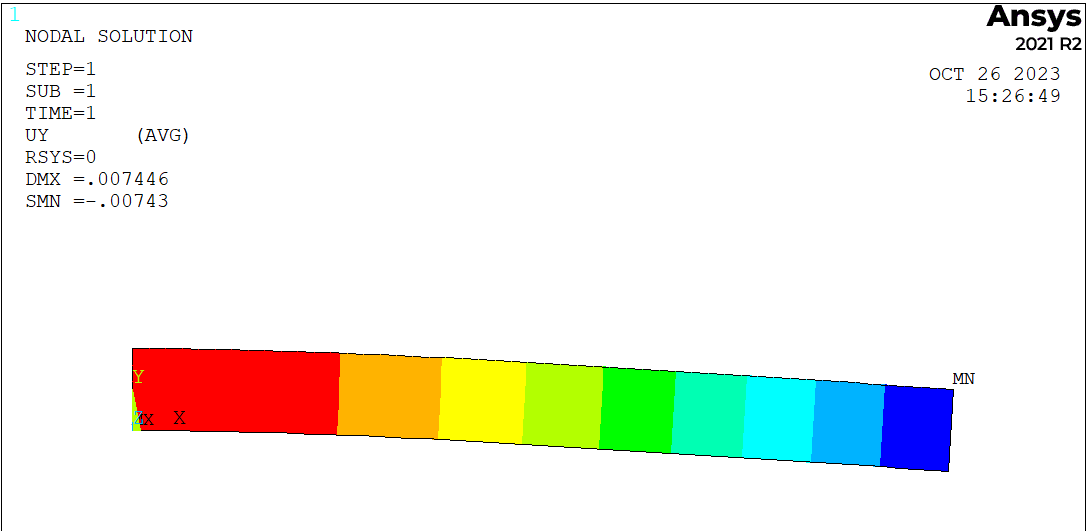
\includegraphics[width=1\textwidth]{p4.PNG}
	\caption{Изгиб балки при разбиении 5 элементами по высоте}
\end{figure}

\pagebreak

\subsection{ Изгиб балки при разбиении 10 элементами по высоте }

\begin{figure}[h]
	\centering
	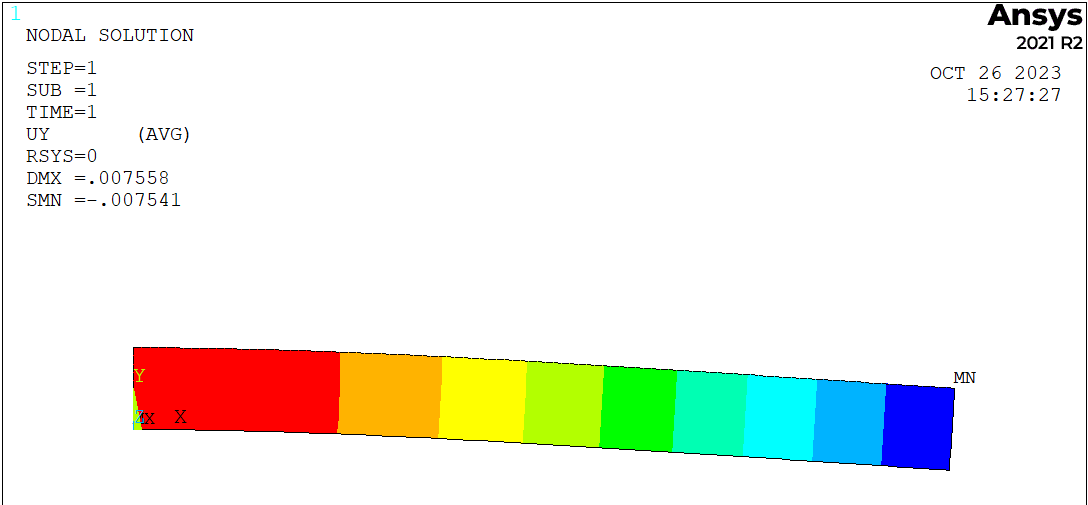
\includegraphics[width=1\textwidth]{p5.PNG}
	\caption{Изгиб балки при разбиении 10 элементами по высоте}
\end{figure}

\pagebreak
    
    \section { График расчета изгиба балки при различном разбиении области двумерными
    	конечными элементами }
    \begin{figure}[h]
    	\centering
    	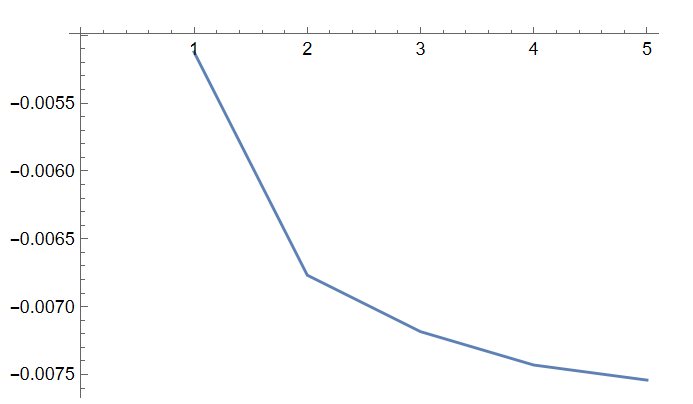
\includegraphics[width=1\textwidth]{graph.PNG}
    	\caption{Расчет изгиба балки при различном разбиении области двумерными
    		конечными элементами (1, 2, 3, 5, 10 элементов по высоте).}
    \end{figure}

\section {Заключение}

В ходе работы была решена задача о нагружении балки внешним давлением в МКЭ-пакете ANSYS Mechanical APDL. Исследована зависимость величины решения от числа КЭ. 
При решении задач необходимо разумное число КЭ. Слишком грубая сетка даст неточное решение. Однако слишком мелкая сетка замедляет вычисления. Необходимо выбрать некоторое среднее число КЭ, при котором значение решения практически не изменяется, т.е. <<выходит на полку>>.



\end{document}